\documentclass[specialist,
               substylefile = ../spbu.rtx,
               subf,href,colorlinks=true, 12pt]{disser}

\usepackage[usenames,dvipsnames,svgnames,table]{xcolor}

\usepackage[a4paper,
            mag=1000, includefoot,
            left=3cm, right=1.5cm, top=2cm, bottom=2cm, headsep=1cm, footskip=1cm]{geometry}
\usepackage[T2A]{fontenc}
\usepackage[utf8]{inputenc}
\usepackage[english,russian]{babel}

% \let\bibfont\relax
\usepackage[style=gost-numeric]{biblatex}
\addbibresource{../biblio-u.bib}

\ifpdf\usepackage{epstopdf}\fi

\usepackage{multirow}
\usepackage{enumitem}

% Точка с запятой в качестве разделителя между номерами цитирований
%\setcitestyle{semicolon}

% Использовать полужирное начертание для векторов
% \let\vec=\mathbf

% Включать подсекции в оглавление
\setcounter{tocdepth}{2}

\usepackage{graphicx}
\graphicspath{ {../media/} }

\usepackage[ruled,vlined]{algorithm2e}

\usepackage[intlimits]{amsmath}
\usepackage{amsfonts}
\usepackage{amssymb}
\usepackage{amsthm}
\usepackage{mathrsfs}

\usepackage{hyperref}
\newtheorem{theorem}{Теорема}
\newcommand{\E}{\mathrm{E}}
\newcommand{\vfi}{\varphi}
\newcommand{\eps}{\varepsilon}
\newcommand{\prob}[1]{\mathrm{P}\left(#1\right)}
\newcommand{\R}{\ensuremath{\mathbb{R}}}
\newcommand{\Tau}{\ensuremath{\mathcal{T}}}
\newcommand{\GothB}{\mathfrak{B}}
\newcommand{\norm}[1]{\left\lVert#1\right\rVert}
\newcommand{\abs}[1]{\left\lvert#1\right\rvert}
\newcommand{\Vhat}{\hat{V}}
\newcommand{\vhat}{\hat{v}}
\newcommand{\maxset}[1]{\max\left\lbrace#1\right\rbrace}
\newcommand{\deltat}{\Delta t}
\DeclareMathOperator{\correlation}{cor}
\newcommand{\corr}[2]{\correlation\left(#1, #2\right)}
\DeclareMathOperator*{\argmax}{arg\,max}
\DeclareMathOperator*{\argmin}{arg\,min}
\DeclareMathOperator{\dd}{d}

% \usepackage[fixlanguage]{babelbib}
% \selectbiblanguage{russian}
% \setbtxfallbacklanguage{russian}


%----------------------------------------------------------------
\begin{document}

%
% Титульный лист на русском языке
%

% Название организации
\institution{%
    Санкт-Петербургский государственный университет \\
    Прикладная математика и информатика \\
    Статистическое моделирование
}

\title{Отчет о научно-исследовательской работе}

% Тема
\topic{\normalfont\scshape%
    Методы оценки Американского опциона}

% Автор
\author{Миллер Анастасия Александровна}

% Научный руководитель
\sa       {С.\,М.~Ермаков}
\sastatus {д.\,ф.-м.\,н., профессор}

% Город и год
\city{Санкт-Петербург}
\date{\number\year}

\begin{large}
\maketitle
\end{large}

\tableofcontents

\intro
В работе рассмотрены основные подходы к оценке стоимости Американских опционов и приведено их сравнение между собой (как теоретическое, так и на численных примерах). Приведены некоторые методы снижения дисперсии: классические метод противоположных переменных и метод контрольных переменные и более редко используемый метод рандомизированного квази Монте-Карло.

Основной вопрос, исследованный в этом семестре --- применение метода квази Монте-Карло к оценкам и сравнение его с основными методами снижения дисперсии (глава \ref{cha:quasi_monte_carlo}).

В главе \ref{cha:option_price_estimation_problem} описана задача оценки Американских опционов (в секции \ref{sec:option_price}) и приведены основные методы её решения (случайные деревья, стохастические сетки и линейная регрессия, раздел \ref{sec:estimators}). 
% Глава \ref{cha:variance_reduction} содержит описание методов снижения дисперсии оценок, в частности, применение квази Монте-Карло. 
В главе \ref{cha:quasi_monte_carlo} более подробно разобрана теория квази Монте-Карло и приведены обоснования для выбора размерности квазислучайной последовательности. В большинстве секций теоретические сведения подкреплены демонстрацией вычислений на конкретных примерах.

\chapter{Задача оценки стоимости Американского опциона} % (fold)
\label{cha:option_price_estimation_problem}

Опцион --- это широко распространённый вторичный (производный) финансовый инструмент. Опцион является контрактом между продавцом опциона и покупателем опциона о том, что покупатель имеет право, но не обязательство, купить (в случае опциона на покупку, call option) или продать (в случае опциона на продажу, put option) указанный в контракте базовый актив по заранее оговорённой цене в определённый контрактом момент в будущем или на протяжении определённого отрезка времени. Продавца опциона контракт обязует совершить ответную продажу (для опциона на покупку) или покупку (для опциона на продажу) в случае, если покупатель пожелает исполнить своё право. Реализация такой сделки называется \emph{исполнением опциона}.

Различают опционы европейского и американского типа. Опцион европейского типа выписывается на фиксированный момент времени в будущем, опцион американского типа --- на отрезок времени. Промежуточный вариант, когда опцион может быть исполнен только в определённые даты (например, в конце каждого квартала в течение года), часто называют Бермудским опционом.

Исполнение опциона может быть выгодно его владельцу (когда цена базового актива в контракте ниже текущей рыночной в случае опциона на покупку, когда цена базового актива выше текущей рыночной в случае опциона на продаже), поэтому опционный контракт сам по себе тоже имеет стоимость. Ищется стоимость опциона в модели эффективного рынка, то есть такая цена, при которой ни продавец, ни покупатель опциона в среднем не получают прибыли.

\section{Стоимость Американского опциона как случайная величина} % (fold)
\label{sec:option_price}

В случае опциона европейского типа существует решение в замкнутой форме (модель Блэка-Шоулса \cite{Black1973} и её усовершенствования). Оценка Американского опциона является более сложной задачей.

Опцион определяется 
\begin{itemize}[noitemsep,topsep=0pt]
\item своим временем жизни $[0;T]$, 
\item базовым активом $X$ (под $X(t)$ будем подразумевать состояние актива в момент времени $t$, являющееся случайной величиной, под $S(t) = S(X(t))$ --- цену базового актива в момент $t$), на который выписан опцион (список возможных активов на территории Российской Федерации представлен в \cite{fsfr}), 
\item процессом $U(t), t\in [0;T]$, представляющим дисконтированное значение функции выплат (разницы между рыночной стоимостью базового актива и ценой страйк, оговорённой в контракте; значение функции выплат показывает выгоду, получаемую владельцем опциона при исполнении),
\item множеством $\Tau$ моментов времени, в которых возможно исполнить опцион.
\end{itemize} 
Будем также считать, что существует $h_t: U(t) = h_t\left(X(t)\right)$. Тогда для Американского опциона с функцией выплат $h_t\left(X_t\right)$, задача оптимального исполнения --- это задача о нахождении 
\begin{equation}\label{eq:optimal_stopping}
V = \max_{\tau} \E h_\tau\left(X_\tau\right).
\end{equation}

При дискретизации \eqref{eq:optimal_stopping} (принятии предположения о том, что $\Tau$ -- конечное множество $\left\lbrace t_i\right\rbrace_{i=0}^n \in \left[0;T\right], t_0 = 0, t_n = T$) задача обретает эквивалентную формулировку о нахождении $V_0\left(X_0\right)$ для
\begin{equation}\label{eq:option-recursive}\begin{aligned}
			V_m\left(x\right) &= h_m\left(x\right), \\
			V_{i-1}\left(x\right) &= \max\left\lbrace h_{i-1}\left(x\right), \E\left[V_i\left(X_i\right)|X_{i-1}=x\right]\right\rbrace.
\end{aligned}\end{equation}

% section option_price (end)

\section{Оценки} % (fold)
\label{sec:estimators}

Наверное, самый простой способ оценить стоимость Американского опциона --- это промоделировать много вариантов траекторий базового актива, посчитать выплату по опциону в каждом случае и усреднить результаты. Это классический метод Монте-Карло. Как видно из рис.~\ref{fig:classical_methods}, на коротом изображено сравнение результатов работы некоторых из классических методов, дисперсия наивного Монте-Карло для этой задачи слишком велика.

Все предложенные ниже способы --- это различные попытки уменьшить дисперсию наивного варианта путём увеличения числа моделируемых траекторий. 

\begin{figure}[t]
    \centering
	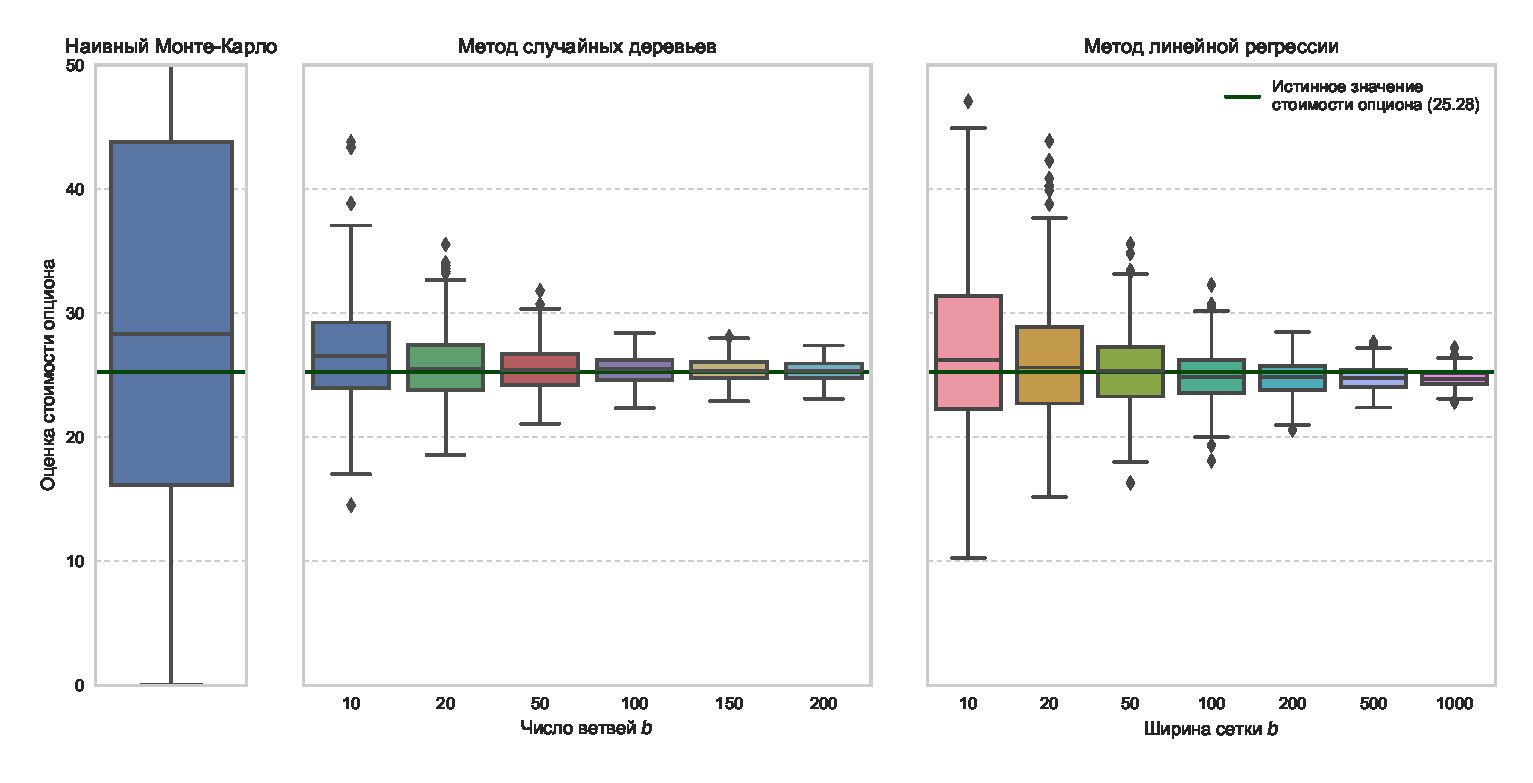
\includegraphics[width=\textwidth]{classical_methods.eps}
	\caption{Оценки стоимости опциона различными классическими методами}
	\footnotesize Опцион на 5 независимых базовых активов. Подробное описание параметров моделирования см.~в~секции~\ref{ssub:random_trees_numerical_results}. Результаты метода случайных деревьев описаны в~\ref{ssub:random_trees_numerical_results}, метода наименьших квадратов --- в секции~\ref{ssub:lsm_numerical_results}.
	\label{fig:classical_methods}
\end{figure}

\subsection{Случайные деревья} % (fold)
\label{sub:tree_estimator}

Метод случайного дерева основан на моделировании цепи $X_0, X_1, \ldots X_n$ состояний актива. Зафиксируем параметр ветвления $b$. Из исходного состояния $X_0$ смоделируем $b$ независимых следующих состояний $X_1^1, X_1^2, \ldots X_1^b$, все с условием $X_0$. Для каждого $X_1^i$ снова смоделируем $b$ независимых последующих состояний $X_2^{i1}, \ldots X_2^{ib}$. На $m$-ом шаге будем иметь $b^m$ состояний, и это и есть источник основного недостатка этого метода --- его экспоненциальной алгоритмической сложности. Схема приведена на рис. \ref{fig:exponential_tree}.
\begin{figure}[b]
    \centering
	\includegraphics{exponential_tree.pdf}
	\caption{Случайное дерево для $b = 3$ и $m = 2$}
	\label{fig:exponential_tree}
\end{figure}

В \cite{Broadie1997} предложены оценки сверху и снизу $\hat{V}_0$ и $\hat{v}_0$ и доказана их состоятельность и асимптотическая несмещённость для $V_0\left(X_0\right)$.
\begin{equation}\label{eq:upper}
\begin{aligned}
	\hat{V}_m^{j_1 \ldots j_m} &= h_m\left(X_m^{j_1 \ldots j_m}\right), \\
	\hat{V}_i^{j_1 \ldots j_i} &= \max \left\lbrace h_i \left( X_i^{j_1 \ldots j_i} \right), \frac{1}{b} \sum_{j = 1}^b \hat{V}_{i+1}^{j_1 \ldots j_i j}\right\rbrace,
\end{aligned}\end{equation}
\begin{equation}\label{eq:lower}
\begin{aligned}
	\hat{v}_m^{j_1 j_2 \cdots j_m} &= h\left( X_m^{j_1 j_2 \cdots j_m}\right), \\
	\hat{v}_{ik}^{j_1 j_2 \cdots j_i} &= \left\lbrace
			    \begin{array}{l l}
				    h\left( X_i^{j_1 j_2 \cdots j_i}\right), & \, \text{если } \frac{1}{b-1}\sum_{j=1, j\not= k}^b \hat{v}_{i+1}^{j_1 j_2 \cdots j_i j} \leq h\left(X_i^{j_1 j_2 \cdots j_i}\right), \\
				    \hat{v}_{i+1}^{j_1 j_2 \cdots j_i k}, & \, \text{иначе}
			    \end{array}\right. \\
	\hat{v}_i^{j_1 j_2 \cdots j_i} &= \frac{1}{b}\sum_{k=1}^b \hat{v}_{ik}^{j_1 j_2 \cdots j_i}.
\end{aligned}\end{equation}

Алгоритм прост в реализации и нетребователен по памяти: при реализации обходом в глубину память ограничена $O(m)$. Основной недостаток -- экспоненциальная сложность по времени: обойти всё дерево получится за $O(m^b)$.

\subsubsection{Численные результаты} % (fold)
\label{ssub:random_trees_numerical_results}

Для большинства упомянутых методов в работе представлены численные результаты. Алгоритмы были реализованы на языке Python с использованием библиотек NumPy и SciPy~\cite{Jones2001}.

Результаты работы всех реализованных алгоритмов приведены для одного примера: колл опцион на максимум из 5 независимых активов, выписанный на $T = 3$ года, который можно исполнить 4 раза в течение года: в момент получения 0, $T/ 3$, $2T / 3$ и в момент окончания срока действия $T$. Платёжная функция опциона $$h_t(X_t) = \left(\max(X_t) - K\right)^+, X_t\in \mathbb R^5.$$
Стартовая цена каждого из активов $S_0 = 100$, цена страйк $K = 100$. Поведение опциона моделируется с помощью геометрического броуновского движения (подробное объяснение есть в \cite[стр.~1336]{Broadie1997}), безрисковая процентная ставка $r = 5\%$, дивидендная ставка $\delta = 10\%$ и волатильность стоимости актива $\sigma = 20\%$.

Это более содержательный пример, чем одномерные опционы, на нём видны некоторые проблемы, которые для одномерных опционов просто не существуют (например, становится нетривиальной задачей разбиение пространства состояний базового актива на ячейки одинаковой вероятности\footnote{Такой вариант понижения вычислительной сложности метода случайных деревьев рассматривался автором, но содержательных результатов для многомерного случая получить не удалось.}). Для этого примера можно найти референсные значения в опубликованных работах (\cite[стр.~57]{Broadie2004}~--~для указанных выше параметров, \cite[табл.~5, стр.~1340]{Broadie1997}~--~для~$T=1$).

Для метода случайных деревьев была вычислена оценка сверху на стоимость опциона $\Vhat_0$ \eqref{eq:upper}. Результаты представлены на рис.~\ref{fig:classical_methods} и в табл.~\ref{tbl:random_tree_estimators}. Результаты в таблице посчитаны по 500 испытаниям. Если обозначить результат $i$-го испытания за $\Vhat_i$, $n=500$, то обозначения в таблице расшифровываются следующим образом:
\begin{equation}\label{eq:table_labels}
\begin{aligned}
\Vhat &= \frac{1}{n}\sum_{i=1}^n \Vhat_i \\
\mathrm{sd}\Vhat &= \sqrt{\frac{1}{n}\sum_{i=1}^n \left(\Vhat_i - \Vhat\right)^2} \\
\mathrm{se}\Vhat &= \sqrt{\frac{1}{n}\sum_{i=1}^n \left(\Vhat_i - V\right)^2} \\
\mathrm{Bias}\Vhat &= \left(\mathrm{se}\Vhat\right)^2 - \left(\mathrm{sd}\Vhat\right)^2
\end{aligned}
\end{equation}
\begin{table}
	% \renewcommand{\arraystretch}{0.75}
	\centering
	\caption{Оценки методом случайных деревьев}
	\begin{tabular}{rrrrr}
		$b$&$\Vhat$&$\mathrm{sd}\Vhat$&$\mathrm{se}\Vhat$&$\mathrm{Bias}\Vhat$\\\hline
		10&26.691&4.145&4.378&1.991\\
		20&25.690&2.743&2.774&0.168\\
		50&25.499&1.830&1.843&0.048\\
		100&25.419&1.163&1.171&0.019\\
		150&25.379&0.929&0.935&0.010\\
		200&25.273&0.891&0.892&0.000\\
	\end{tabular}
	\label{tbl:random_tree_estimators}

	\footnotesize
	Результаты приведены для числа ветвей $b = 10, 20, 50, 100, 150, 200$.\\\vspace{-0.3\baselineskip}Расшифровку обозначений см. в выражении~\eqref{eq:table_labels}.
\end{table}

% subsubsection random_trees_numerical_results (end)

% subsection tree_estimator (end)

\subsection{Стохастические сетки} % (fold)
\label{sub:mesh_estimator}

Метод стохастической сетки также предлагает оценки сверху и снизу для решения \eqref{eq:option-recursive}, но принцип построения оценок несколько отличается от рассматриваемых мною оценок по случайному дереву.

Из начального состояния $X_0$ для оценки опциона с $m$ моментами исполнения, равноотстоящими во времени от 0 до $T$, зададим сетку $X_n^i, n\in 1\mathbin{:}m, i \in 1\mathbin{:}b$, узлы которой --- реализации случайной величины с плотностью $p_{0, n}(X_0, \cdot)$ (маргинальные плотности; также рассматриваются средние плотности), а $p_{k, n}(x, y) = \prob{X_n = y \middle\vert X_k = x}$. Тогда определяется $\rho_{n, j}(x, y) = p_{n-1, n}(x, y) / p_{0, n}(X_0, y)$, сокращённые обозначения $\rho_{n, j}(i, j) = \rho_{n, j}(X_{n-1}^i, X_n^j)$ и оценка в каждом узле сетки
$$\hat Y_n(i) = \max\left\lbrace h_n(i), \frac{\sum_j \rho_{n+1}(i, j) \hat Y_{n+1}(j)}{\sum_j \rho_{n+1}(i, j)} \right\rbrace.$$

Иллюстрация взаимоотношений между узлами сетки приведена на рис.~\ref{fig:stochastic_mesh}. Тогда оценка справедливой стоимости опциона --- это $$\hat Y_0 = \max\left\lbrace h_0(X_0), \frac{\sum_j \rho_{1}(X_0, X_1^j) \hat Y_{1}(X_1^j)}{\sum_j \rho_{1}(X_0, X_1^j)} \right\rbrace.$$

\begin{figure}[t]
    \centering
	\includegraphics{stohastic_mesh_vector.eps}
	\caption{Стохастическая сетка для $b = 5$ и $m = 3$}
	\label{fig:stochastic_mesh}
\end{figure}

Этот метод работает гораздо быстрее, чем метод случайных деревьев: сложность и по времени, и по памяти составляет $O(mb)$. Недостатком являются трудоёмкие вычисления в многомерном случае: в отличие от случайного дерева, для обсчёта которого нужно лишь уметь вычислить $h_t(X_t)$ (для традиционного примера максимум-опциона на покупку $h_t(X_t) = \left(\max(X_t) - K\right)^+$, если $X_t$ -- вектор стоимостей базовых активов в момент $t$), для стохастических сетей нужно точно вычислять $\rho_n(i, j)$.

% subsection mesh_estimator (end)

\subsection{Метод наименьших квадратов} % (fold)
\label{sub:least_squares}

Несколько отличающийся от двух предыдущих вариант --- метод оценки с помощью линейной регрессии. Согласно формулировке \eqref{eq:option-recursive}, в каждый момент $t$ мы хотим знать математическое ожидание стоимости удержания (неисполнения) опциона при условии его текущего состояния. Классический инструмент для оценки условного математического ожидания --- это линейная регрессия. Будем оценивать стоимость удержания опциона следующим образом:

\begin{equation}\label{eq:lsm_continuation}
\E\left(V_i(X_i)\middle\vert X_{i-1} = x\right) \approx \sum_{r=1}^M \beta_{ir} \psi_r(x) = \beta_i^\mathsf{T}\psi(x).
\end{equation}
Здесь $\psi(x) = \left(\psi_1(x), \dots, \psi_M(x)\right)^\mathsf{T}$ --- это набор регрессоров, используемых для построения оценки. В оригинальной статье использовались полиномы Лагера (\cite{Longstaff2001}, секция~2.2 на стр.~122) и для построения регрессии использовались только те траектории, на которых опцион в $i-1$-й момент времени находился в деньгах.

Мы используем сетку, схожую с той, что была в методе стохастической сетки: моделируем несколько траекторий, тем самым получая нужный набор примеров (см. рис.~\ref{fig:least_squares}). Коэффициенты $\beta$ оцениваются по методу наименьших квадратов. 

\begin{figure}[t]
    \centering
	\includegraphics{stohastic_mesh_vector_phase_0.eps}
	\caption{Стохастическая сетка для метода наименьших квадратов, $b = 5$ и $m = 3$}
	\label{fig:least_squares}
\end{figure}

Для каждого узла сетки мы можем оценить стоимость удержания опциона по выражению \eqref{eq:lsm_continuation}, и тем самым понять, было ли оптимальным решением исполнить опцион в этот момент. После того, как установлены моменты оптимального исполнения опциона, для каждой из исходных траекторий, составлявших сетку, можно установить стоимость опциона на этой траектории, как выплату, полученную в момент оптимального исполнения. Итоговая стоимость опциона оценивается усреднением по всем траекториям. Более формально эта процедура изложена в алгоритме~\ref{alg:least_squares_estimation}.

\begin{algorithm}[h]
	\SetAlgorithmName{Алгоритм}{алгоритм}{Список алгоритмов}
	\SetKwInput{KwData}{Входные данные}
	\SetKwInput{KwResult}{Результат}
	\SetKw{KwTo}{до}\SetKwFor{For}{Для}{\string:}{}%
	\KwData{сетка из $b$ промоделированных траекторий состояния базового актива $X_n^i, n\in 1\mathbin{:}m, i \in 1\mathbin{:}b$}
	\KwResult{$\Vhat$ -- оценка стоимости опциона}
	
	положим стоимость опциона равной выплате по нему в последний момент исполнения:\\$C_i \leftarrow h_{t_m}\left(X_m^i\right)$, $C = \left(C_1, \dots, C_b\right)^{\mathsf T}$\;
	\For{$n\leftarrow m-1$ \KwTo $1$}{
		дисконтируем стоимость опциона: $C \leftarrow e^{-r\deltat} \cdot C$\;
		$X_i \leftarrow S_n^i$, $X = \left(X_1, \dots, X_b\right)^{\mathsf T}$\;
		выплаты по исполнении опциона $P_i \leftarrow h_{t_n}\left(X_n^i\right)$, $P = \left(P_1, \dots, P_b\right)^{\mathsf T}$\;
		строим линейную регрессию $C$ на $X$ через набор базисных функций $\psi$ по всем тем примерам, где опцион в деньгах:\\ $\beta \leftarrow \argmin_{\beta'\in\R^M} \norm{\left({\beta'}^\mathsf{T}\psi(X_i) - C_i\right)_{\left\{i \middle\vert P_i > 0\right\}}}^2$\;
		стоимость удержания опциона $H_i = \beta^\mathsf{T}\psi(X_i)$\;
		\For{всех $i$ таких, что $P_i > H_i$}{
			$C_i \leftarrow P_i$\;
		}
	}
	$\Vhat \leftarrow \frac{1}{b}\sum_{i=1}^b C_i$

	\caption{Оценка стоимости опциона по методу наименьших квадратов}
\label{alg:least_squares_estimation}
\end{algorithm}

% В результате мы получаем следующий алгоритм оценки:

% \begin{equation}
% 	\begin{aligned}
% 	\Vhat_m^j &= h_m(X_m^j), \quad \hat\beta_i = \argmin_{\beta\in\R^m} \norm{\left(\beta^\mathsf{T}\psi(X_i^j) - \Vhat_{i+1}^j\right)_{j=1}^b}^2 \\
% 		\Vhat_i^j &= \maxset{h_i(X_i^j), \hat \beta_i^\mathsf{T}\psi(x)},\;\; \Vhat_0 = \frac{1}{b}\sum_{j=1}^b V_1^j\end{aligned}\label{eq:least_squares}
% \end{equation}

В \cite{Glasserman2004} указано, что метод наименьших квадратов можно считать частным случаем метода стохастической сетки со специальным выбором весов. Тем не менее, часто эти подходы рассматриваются по отдельности.

\subsubsection{Численные результаты} % (fold)
\label{ssub:lsm_numerical_results}

Метод наименьших квадратов был реализован для $\psi_1(x) = x, \psi_2(x) = x^2$. Результаты представлены на рис.~\ref{fig:classical_methods} и в табл.~\ref{tbl:lsm_estimators}.

\begin{table}
	% \renewcommand{\arraystretch}{0.75}
	\centering
	\caption{Оценки методом наименьших квадратов}
	\begin{tabular}{rrrrr}
		$b$&$\Vhat$&$\mathrm{sd}\Vhat$&$\mathrm{se}\Vhat$&$\mathrm{Bias}\Vhat$\\\hline
		10&26.870&6.324&6.521&2.527\\
		20&25.957&4.774&4.822&0.459\\
		50&25.312&2.877&2.877&0.001\\
		100&24.965&2.106&2.129&0.099\\
		200&24.795&1.480&1.557&0.235\\
		500&24.772&0.918&1.050&0.258\\
		1000&24.731&0.636&0.840&0.301\\
	\end{tabular}
	\label{tbl:lsm_estimators}

	\footnotesize
	Результаты приведены для ширины сетки $b = 10, 20, 50, 100, 200, 500, 1000$.\\\vspace{-0.3\baselineskip}Расшифровку обозначений см. в выражении~\eqref{eq:table_labels}.
\end{table}


% subsubsection lsm_numerical_results (end)

% subsection least_squares (end)



% section estimators (end)

% % chapter option_price_estimation_problem (end)

% \chapter{Методы снижения дисперсии} % (fold)
% \label{cha:variance_reduction}

% \section{Противоположные переменные} % (fold)
% \label{sec:antithetic_variables}

% % section antithetic_variables (end)

% \section{Контрольные переменные} % (fold)
% \label{sec:control_variates}

% % section control_variates (end)

% \section{Квази Монте Карло} % (fold)
% \label{sec:quasi_monte_carlo}

% % section quasi_monte_carlo (end)

% chapter variance_reduction (end)

\chapter{Квази Монте Карло} % (fold)
\label{cha:quasi_monte_carlo}

\section{Основные понятия} % (fold)
\label{sec:quasi_mc_definition}

Отклонением (star discrepancy, $D^*$) последовательности из $N$ $d$-мерных случайных векторов в гиперкубе $\left[0;1\right]^d$ называют величину
$$D_N^* = D_N^*\left(X_1, \dots, X_N\right) = \sup_{v = (v_1, \dots, v_d) \in \left[0;1\right]^d} N \abs{\frac{\#\left\{ X_i \in J(v) \right\}}{N} - \prod_{j = 1}^d v_j},$$
где $J(v) = \left[0; v_1\right) \times \dots \times \left[0; v_d\right)$.

В случае, когда последовательность $\left\{ X_i\right\}_{i=1}^\infty$ такова, что $\forall N \: D_N^* \leq C_s \frac{(\ln N)^s}{N}$, последовательность называется последовательностью с низким отклонением (или с низким дискрепансом). С вычислительной точки зрения она представляет интерес из-за неравенства Коксмы-Хлавки: для интеграла, оцененного по этой последовательности, верно утверждение

\begin{equation}\label{eq:koksma-hlawka}
\abs{\int_{\left[0;1\right]^d} f(X) \dd X - \frac{1}{N}\sum_{i=1}^N f(X_i)} \leq \mathrm{Var}f\cdot \frac{D_N^*\left(X_1, \dots, X_N\right)}{N},
\end{equation}
где $\mathrm{Var}f$ -- вариация функции в смысле Харди-Краузе. При $N\to\infty$ эта оценка погрешности лучше, чем оценка погрешности классического Монте-Карло.
% section quasi_mc_definition (end)

\section{Рандомизация} % (fold)
\label{sec:randomization}

Неравенство Коксмы-Хлавки \eqref{eq:koksma-hlawka} с точки зрения оценивания погрешности вычислений обладает двумя существенными недостатками: $\mathrm{Var}f$ сложно вычислить (особенно в тех случаях, когда функция вообще плохо описывается в явном виде, как в задаче оценки опциона) и оно даёт очень консервативную оценку (настоящая погрешность обычно существенно меньше, чем эта верхняя граница). Тогда как для большинства приложений нам необходим инструмент, позволяющий хорошо и быстро оценивать, насколько сильно ошибается оценка. Такой, как доверительные интервалы в методе Монте-Карло.

Одно из решений этой задачи --- рандомизация квазислучайных последовательностей. К последовательности применяется некоторое случайное преобразование, после которого мы имеем дело уже не с детерминированной последовательностью, а с реализациями некоторой случайной величины.

Основные типы преобразований --- это случайный сдвиг (см.~\cite{Tuffin2004}) и случайные перестановки (см.~\cite{Owen1995}). Мы будем рассматривать случайный сдвиг как более удобный с точки зрения анализа вариант.

Квази Монте-Карло последовательность $\left\{ X_i\right\}_{i \in \mathbb N} \subset \left[0;1\right]^d$, рандомизированная с помощью случайного сдвига --- это последовательность $\left\{ \hat X_i = X_i + \Xi_i \mod 1\right\}_{i \in \mathbb N} \subset \left[0;1\right]^d$, где $\Xi_i \sim \mathrm U\left[0;1\right]^d$. В случае, когда каждое $\hat X_i$ получено с помощью своей собственной реализации $\Xi_i$, результат ничем не отличается от стандартного Монте-Карло. В случае, когда последовательность длины $N$ делится на $h$ групп одинаковой длины $H = N / h$ и $\hat X_{\left(k - 1\right)H + l} = X_{\left(k - 1\right)H + l} + \Xi_k, k \in 1\mathbin{:}h, l \in 1\mathbin{:}H$ (то есть все элементы одной группы смещаются одинаково), мы получаем последовательность из независимых между собой групп, которые зависимы внутри себя. При этом внутри каждой из таких групп взаимное расположение точек меняется только на сдвиг на константу, что позволяет нам надеяться, что неравенство Коксмы-Хлавки не будет нарушено и за нами останется выигрыш в дисперсии. Наличие такого выигрыша демонстрируют численные эксперименты в \cite{Tuffin2004}.

% section randomization (end)

\section{Приложение к задаче оценки стоимости Американского опциона} % (fold)
\label{sec:monte_carlo_in_option_pricing}

Как мы уже видели в главе~\ref{cha:option_price_estimation_problem}, вопрос снижения дисперсии при оценивании стоимости Американского опциона очень важен. Несмотря на то, что сама возможность использования квази Монте-Карло в финансовых задачах в целом в литературе упоминается (\cite[глава~5]{Glasserman2004} и ссылки оттуда), подробного разбора метода в приложении к задаче оценки Американского опциона ещё не публиковалось.

В этом разделе освещены некоторые технические аспекты изпользования рандомизированного квази Монте-Карло и анализа его результатов. Также приведены численные результаты, согласно которым оценки, полученные с помощью рандомизированного квази Монте-Карло, действительно имеют меньшую дисперсию, чем оценки, полученные с помощью обычного Монте-Карло.

\subsection{Преобразование в нормальное распределение} % (fold)
\label{sub:uniform_normal_transform}

Квази Монте-Карло обычно рассматривается в контексте задачи интегрирования функции на $\left[0;1\right]^d$, а параллели проводятся с классическим Монте-Карло с использованием распределения $\mathrm U\left[0;1\right]^d$. В финансовых задачах же обычно используются нормальное и логнормальное распределения, но не равномерное. Поэтому первый вопрос, которому стоит уделить внимание --- это вопрос о корректном преобразовании, которое переводило бы последовательность с низким дискрепансом на $\left[0;1\right]^d$ в последовательность с низким дискрепансом по мере нормального распределения. Согласно \cite{Oekten2011}, преобразование Бокса-Мюллера, применённое к <<распрямлённой>> квазислучайной последовательности, применимо в этом случае.

% subsection uniform_normal_transform (end)

\subsection{Выбор размерности} % (fold)
\label{sub:choice_of_dimension}

В контексте задачи многомерного интегрирования, в которой обычно говорится о квази Монте-Карло, размерность пространства, по которому происходит интегрирование, является условием задачи. В случае задачи оценивания опционов ответ на вопрос о том, какой же должна быть размерность квазислучайной последовательности, не столь очевиден.

Во-первых, если исходить из того, что функцией, математическое ожидание которой мы оцениваем, является весь обсчёт сетки или дерева, то размерность интегрируемого пространства --- это конструктивная размерность алгоритма, то есть $\sum_{i=1}^m b^i$ для оценки по случайным деревьям и $mb$ для метода сетки или наименьших квадратов.

В случае сколько-нибудь разумных $m$ и $b$ (например, $m = 3$ и $b = 50$) конструктивная размерность линейных методов уже достаточно высока для квазислучайных последовательностей, а для метода случайных деревьев гораздо выше допустимых пределов. Так, для построения последовательности Холтона размерности 150 нужно получить 150 взаимно простых чисел. В случае, когда мы берём последовательность простых чисел, 150-е из них равно 853. Это означает, что по построению последовательности последняя координата первых её 852 точек будет идти равноотстоящими шагами от 0 до 1, что уже не очень похоже на случайные равномерно распределённые на $\left[0; 1\right]$ числа, и рандомизация сдвигом не исправит ситуацию. Это известный недостаток последовательности Холтона, аналогичные проблемы с большими размерностями имеют и другие квазислучайные последовательности.

Поэтому можно использовать другой подход: взять некоторую достаточно большую размерность $n$, взять последовательность из $k$ квазислучайных чисел $\left(x_1^i, \dots, x_n^i\right)$  этой размерности, распрямить (получится вектор $\left(x_1^1, \dots, x_n^1, x_1^2, \dots, x_n^k\right)$ длины $nk$) и работать с ней как с последовательностью из обычного генератора псевдослучайных чисел.

Третий вариант --- это использование размерности, равной размерности базового актива. В конечном счёте оценка стоимости опциона является комбинацией интегралов по пространству состояний базового актива ($\E\left(V_i(X_i)\middle\vert X_{i-1} = x\right)$), и именно эти интегралы мы оцениваем.

% subsection choice_of_dimension (end)

\subsection{Численные результаты} % (fold)
\label{sub:numerical_results}

На рис.~\ref{fig:halton_estimators} приведены результаты моделирования с использованием рандомизированного квази Монте-Карло для всех трёх вариантов размерности, применённых к методу случайных деревьев. Вариант с конструктивной размерностью алгоритма посчитан только для $b = 10$, так как для б\'oльших значений $b$ посчитать его не представляется возможным. Использована квазислучайная последовательность Холтона, для каждого числа ветвей $b$ и размерности последовательности построено 500 оценок $\hat V_0$, при рандомизации последовательности разделённых в 10 независимых групп. Стоит отметить, что высота ящиков с усами здесь не имеет прямого отношения к дисперсии оценки: наличие внутригрупповой корреляции не позволяет оценить дисперсию стандартными методами.

\subsubsection{Оценка дисперсии рандомизированного квази Монте-Карло} % (fold)
\label{ssub:variance_estimation_QMC}

В случае рандомизированного с помощью случайного сдвига квази Монте-Карло (см.~секцию\,\ref{sec:randomization}) получаемые оценки $\Vhat$ являются одинаково распределёнными, но не независимыми. С использованием обозначений из секции\,\ref{sec:randomization} имеем $N$ оценок, каждая из которых принадлежит одной из $h$ групп. Пусть тогда $\Vhat_{ij}, i\in 1\mathbin{:}h, j \in 1\mathbin{:}H$ обозначает $j$-ю оценку в $i$-й группе. По построению оценки из разных групп независимы, но оценки внутри одной группы имеют ненулевую корреляцию. 

Положим теперь 
$$\Vhat_{i\cdot} = \frac{1}{H}\sum_{j=1}^H \Vhat_{ij}.$$
Оценки $\Vhat_{i\cdot}, i\in 1\mathbin{:}h$ всё так же являются оценками $V$, но уже независимыми друг от друга. В таблицах далее для результатов квази Монте-Карло будем использовать следующие обозначения:
\begin{equation}
\begin{aligned}
	\Vhat &= \frac{1}{n}\sum_{i=1}^n \Vhat_{i\cdot} \\
	\mathrm{sd}\Vhat &= \sqrt{\frac{1}{n}\sum_{i=1}^n \left(\Vhat_{i\cdot} - \Vhat\right)^2} \\
	\mathrm{se}\Vhat &= \sqrt{\frac{1}{n}\sum_{i=1}^n \left(\Vhat_{i\cdot} - V\right)^2} \\
	\mathrm{Bias}\Vhat &= \left(\mathrm{se}\Vhat\right)^2 - \left(\mathrm{sd}\Vhat\right)^2
\end{aligned}
\end{equation}

% subsubsection variance_estimation_QMC (end)

Численные значения оценок и оценки дисперсии для квазислучайных последовательностей различной размерности приведены в табл.~\ref{tbl:halton_estimators}. 


\begin{figure}[h]
    \centering
	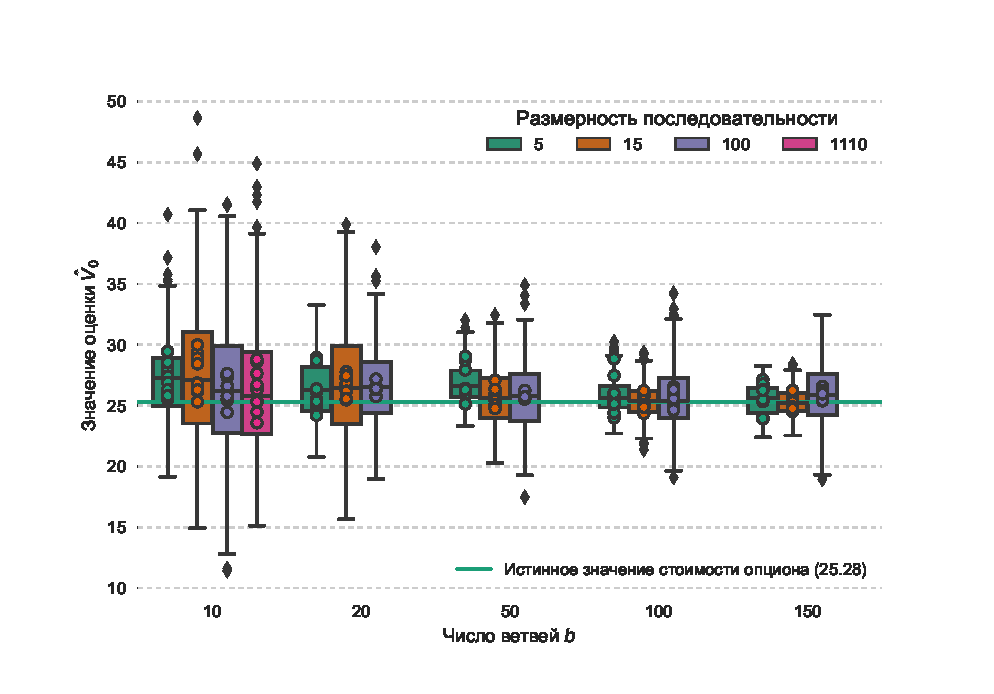
\includegraphics[width=\textwidth]{halton_estimators.eps}
	\caption{Оценки рандомизированными квазислучайными последовательностями}
	\footnotesize Параметры опциона см.~в разделе <<Численные результаты>> секции \ref{ssub:random_trees_numerical_results}. Ящики с усами изображают распределение оценок $\Vhat_{ij}$, точками изображены независимые оценки $\Vhat_{i\cdot}$. Вычисления проводятся методом случайных деревьев.
	\label{fig:halton_estimators}
\end{figure}

\begin{table}
	\renewcommand{\arraystretch}{0.6}
	\centering
	\caption{Оценки, полученные с помощью рандомизированных квазислучайных последовательностей разных размерностей}
	\begin{tabular}{rrrrrr}
		$b$&$d$&$\Vhat$&$\mathrm{sd}\Vhat$&$\mathrm{se}\Vhat$&$\mathrm{Bias}\Vhat$\\[5pt]\hline\\[-5pt]
		\multirow{4}{*}{10}&5&27.159&1.296&2.283&3.533\\
		&15&27.467&1.491&2.647&4.784\\
		&100&26.383&1.014&1.499&1.217\\
		&1110&26.340&1.616&1.932&1.123\\[5pt]
		&5&26.386&1.635&1.974&1.224\\
		20&15&26.719&0.802&1.648&2.072\\
		&100&26.559&0.454&1.357&1.635\\[5pt]
		&5&26.839&1.212&1.974&2.429\\
		50&15&25.686&0.648&0.765&0.165\\
		&100&25.774&0.181&0.526&0.244\\[5pt]
		&5&25.849&1.351&1.466&0.324\\
		100&15&25.416&0.583&0.599&0.019\\
		&100&25.656&0.536&0.654&0.141\\[5pt]
		&5&25.464&1.130&1.145&0.034\\
		150&15&25.291&0.562&0.562&0.000\\
		&100&25.883&0.340&0.692&0.363\\[10pt]
	\end{tabular}
	\label{tbl:halton_estimators}

	\footnotesize
	Результаты приведены для числа ветвей $b = 10, 20, 50, 100, 150$ и размерности квазислучайной последовательности $d = 5, 15, 100, 1110$. Колонка $\Vhat$ содержит усреднённое значение $\Vhat_0$ по 500 испытаниям (рандомизация последовательности Холтона при этом проходила $M = 10$ раз, каждая страта содержит 50 испытаний), в колонке $\sqrt{\mathrm{var} \Vhat}$ приведены значения оценки стандартного отклонения (для описания подсчётов см.~приложение~\ref{cha:bootstrap_variance_estimation}).
\end{table}

Можно заметить, что разультаты с размерностью 100 имеют значительно меньшую дисперсию, чем результаты с размерностью 5. \textcolor{red}{Остаётся открытым вопрос о выборе размерности, доставляющей наименьшую дисперсию}.

Сравнение рандомизированного квази Монте-Карло (размерности $d = b(m-1) = 15$ -- количество случайных величин, необходимых для моделирования одной траектории) с классическим Монте-Карло приведено на рис.~\ref{fig:quasi_vs_common_mc} и в табл.~\ref{tbl:quasi_vs_common_mc}. На рис.~\ref{fig:quasi_vs_common_mc} видно, что размах <<сырых>> данных у квази Монте-Карло размерности 15 шире, чем у стандартного Монте-Карло (этот размах изображён с помощью ящиков с усами). Но после приведения квази Монте-Карло к независимым случайным величинам (изображённым с помощью точек) оценки с помощью квази Монте-Карло имеют гораздо меньую дисперсию, чем обычный Монте-Карло. Это хорошо видно в табл.~\ref{tbl:quasi_vs_common_mc}.

% \paragraph{Проверка значимости} 

% Является ли наблюдаемая на графиках разница в дисперсии статистически значимой? Здесь важно помнить, что оценка, с которой мы сейчас работаем, является оценкой сверху. Поэтому имеет смысл проверять отдельно, меньше ли у квази Монте-Карло дисперсия и меньше ли у квази Монте-Карло отклонение от среднего.

% Обозначим полученные в ходе испытаний оценки как $v_1^Q, \dots, v_N^Q$ для оценок по квазислучайным числам и $v_1^P, \dots, v_N^P$ для оценок по псевдослучайным числам. В проведённом эксперименте $N = 500$. Обозначим также $\bar v^Q = \frac{1}{N}\sum_{i=1}^N v_i^Q$ и $\bar v^P = \frac{1}{N}\sum_{i=1}^N v_i^P$.

% Проверим нулевую гипотезу о том, что случайно взятое отклонение от среднего $\left(v_i^Q - \bar v^Q\right)^2$ равновероятно больше или меньше случайно взятого отклонения от среднего $\left(v_i^P - \bar v^P\right)^2$, то есть
% $$H_0: \prob{\left(v_i^Q - \bar v^Q\right)^2 > \left(v_i^P - \bar v^P\right)^2} = \prob{\left(v_i^Q - \bar v^Q\right)^2 < \left(v_i^P - \bar v^P\right)^2}.$$
% Это нулевая гипотеза $U$-теста Манна-Уитни. Будем проверять её против альтернативы $H_0: \prob{\left(v_i^Q - \bar v^Q\right)^2 > \left(v_i^P - \bar v^P\right)^2} < \prob{\left(v_i^Q - \bar v^Q\right)^2 < \left(v_i^P - \bar v^P\right)^2}$. Тогда вероятность получить такое и более отклоняющееся от среднего значение статистики, как то, которое получается по имеющейся выборке (то есть $p$-value), равна 0.0017. Таким образом, можно отвергать $H_0$ и с уверенностью говорить, что дисперсия оценок по квазислучайным числам меньше.



% Для отклонений оценки от среднего была проверена гипотеза $U$-теста Манна-Уитни (верно ли, что случайно взятое отклонение от среднего оценки, вычисленной по квазислучайным числам, будет с одинаковой вероятностью больше или меньше случайно взятого отклонения от среднего оценки, вычисленной по псевдослучайной последовательности) против альтернативы о том, что отклонения оценок по квазислучайным числам меньше отклонений по псевдослучайным числам. $p$-value гипотезы равно 0.0017, так что дисперсия квази Монте-Карло статистически значимо меньше дисперсии обычного Монте-Карло в этом численном эксперименте.

\begin{figure}[h]
    \centering
	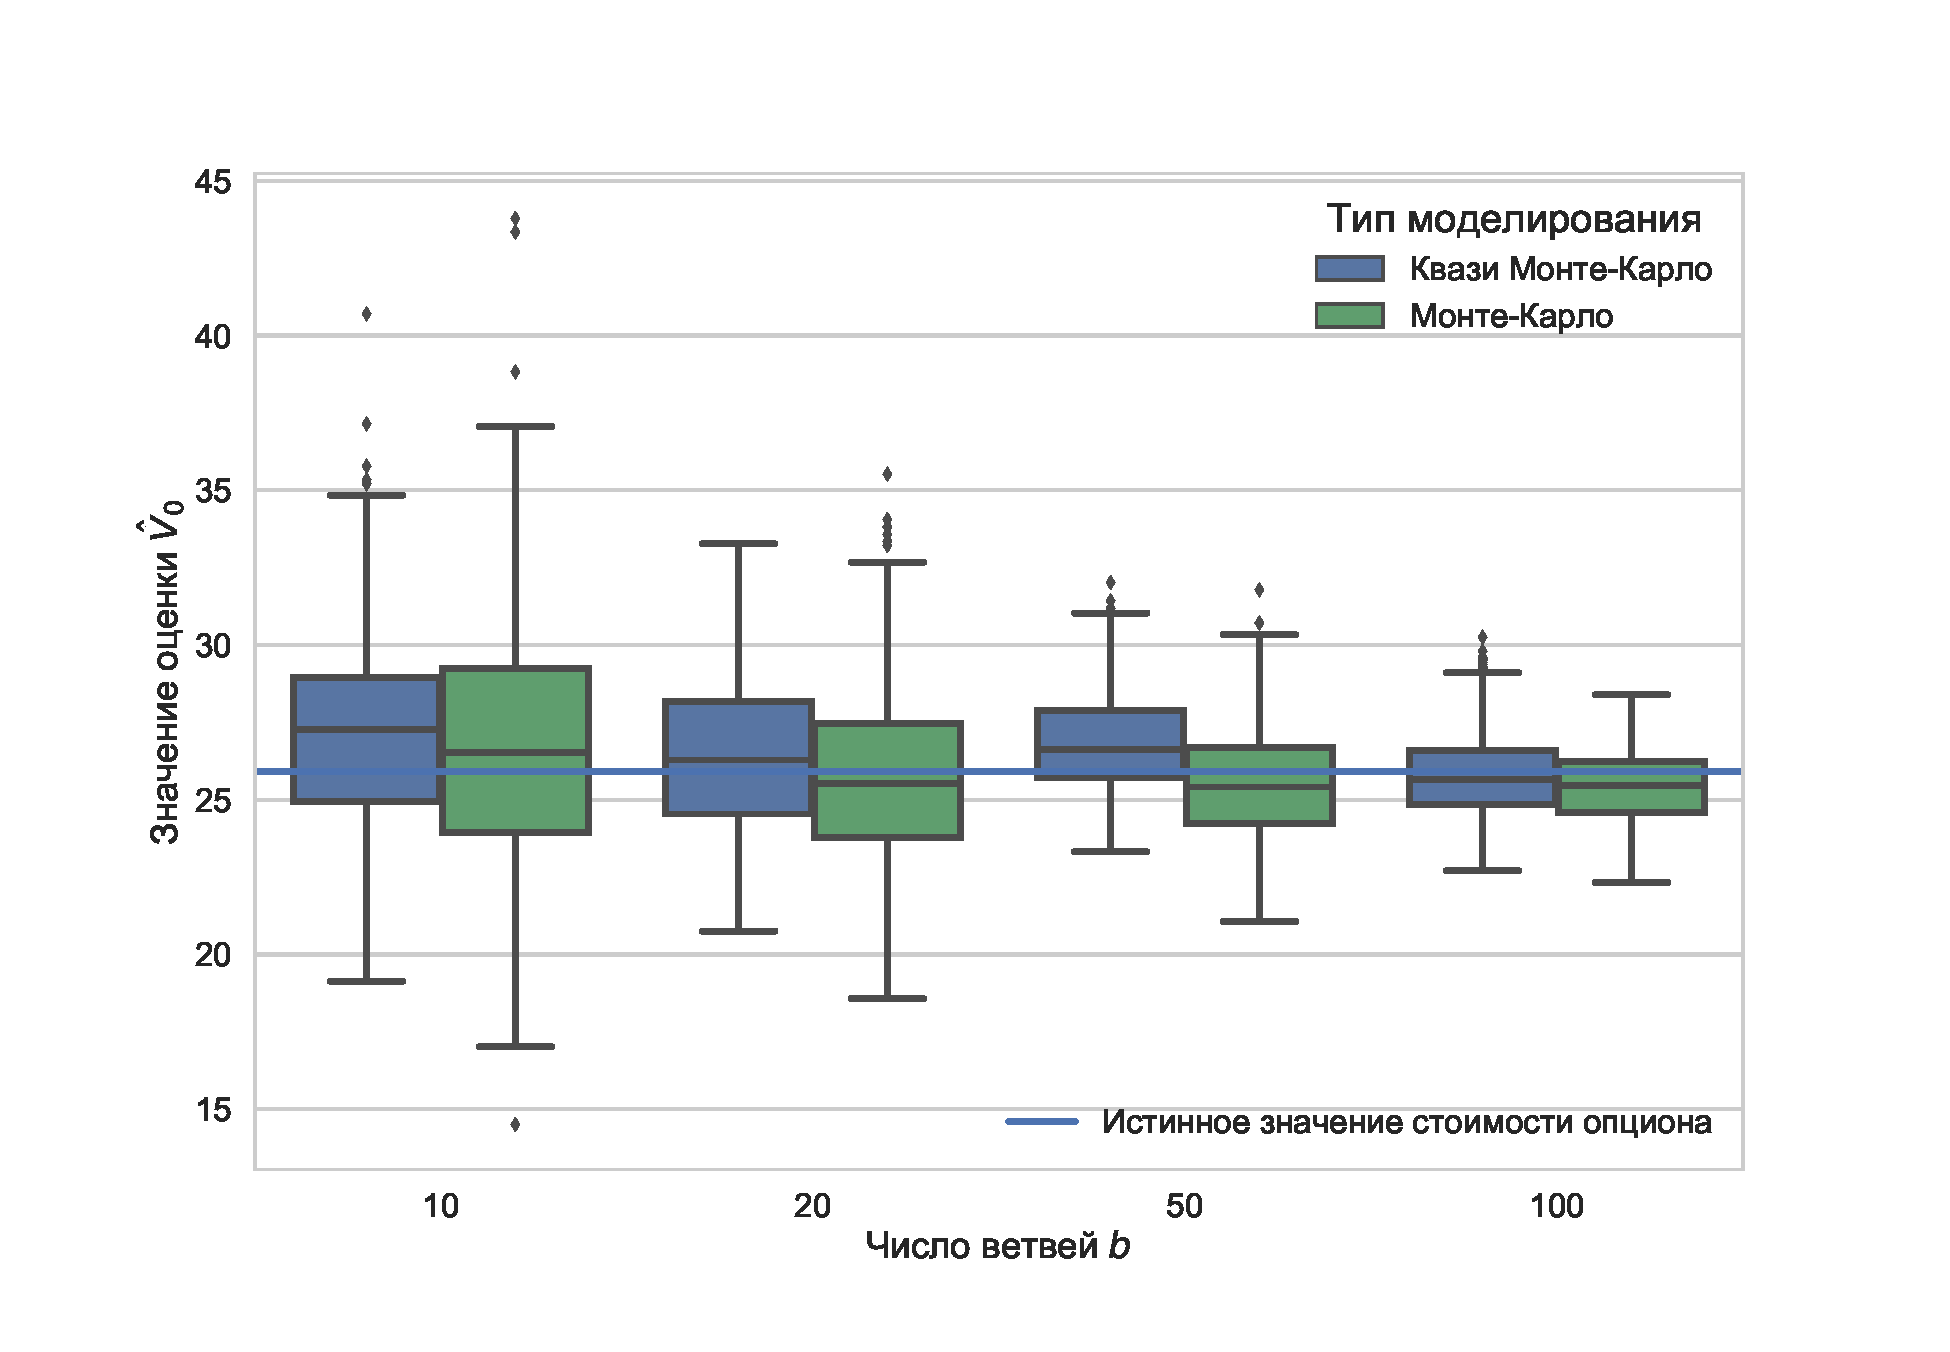
\includegraphics[width=\textwidth]{quasi_vs_common_mc.eps}
	\caption{Сравнение рандомизированной квазислучайной последовательности и стандартного метода}
	\footnotesize Параметры опциона см.~в разделе <<Численные результаты>> секции \ref{ssub:random_trees_numerical_results}. Ящики с усами изображают распределение оценок $\Vhat_{ij}$. Размерность последовательности для квази Монте-Карло $d = b(m-1) = 15$. Вычисления проводятся методом случайных деревьев.
	\label{fig:quasi_vs_common_mc}
\end{figure}

\begin{table}
	\renewcommand{\arraystretch}{0.6}
	\centering
	\caption{Оценки, полученные с помощью рандомизированных квазислучайных последовательностей разных размерностей}
	\begin{tabular}{rrrrrr}
		$b$&тип последовательности&$\Vhat$&$\mathrm{sd}\Vhat$&$\mathrm{se}\Vhat$&$\mathrm{Bias}\Vhat$\\[5pt]\hline\\[-8pt]

		\multirow{2}{*}{10}&Монте-Карло&26.691&4.145&4.378&1.991\\
		&Квази Монте-Карло&27.467&1.491&2.647&4.784\\[5pt]
		\multirow{2}{*}{20}&Монте-Карло&25.690&2.743&2.774&0.168\\
		&Квази Монте-Карло&26.719&0.802&1.648&2.072\\[5pt]
		\multirow{2}{*}{50}&Монте-Карло&25.499&1.830&1.843&0.048\\
		&Квази Монте-Карло&25.686&0.648&0.765&0.165\\[5pt]
		\multirow{2}{*}{100}&Монте-Карло&25.419&1.163&1.171&0.019\\
		&Квази Монте-Карло&25.416&0.583&0.599&0.019\\[5pt]
		\multirow{2}{*}{150}&Монте-Карло&25.379&0.929&0.935&0.010\\
		&Квази Монте-Карло&25.291&0.562&0.562&0.000\\[10pt]
	\end{tabular}
	\label{tbl:quasi_vs_common_mc}

	\footnotesize
	Результаты приведены для числа ветвей $b = 10, 20, 50, 100, 150$ и псевдослучайных и квазислучайных (размерности $d = b(m-1) = 15$) последовательностей. Колонка $\Vhat_0$ содержит усреднённое значение $\Vhat_0$ по 500 испытаниям (рандомизация последовательности Холтона при этом проходила $M = 10$ раз, каждая страта содержит 100 испытаний), в колонке $\mathrm{sd}\Vhat_0$ приведены значения стандартного отклонения.
\end{table}

% subsection numerical_results (end)

% section monte_carlo_in_option_pricing (end)

% chapter quasi_monte_carlo (end)

\conclusion

В этом семестре я исследовала вопрос о применимости рандомизированных квазислучайных последовательностей к задаче оценивания Американского опциона. Полученные результаты (см.~\ref{sub:numerical_results}) показывают, что квазислучайные последовательности могут быть применены в этой задаче и дают статистически значимый прирост точности. 

Пока остался за рамками остался вопрос о комбинировании этой техники с такими приёмами уменьшения дисперсии, как противоположные переменные и контрольные переменные, но результаты исследования этого вопроса будут включены в ВКР. Ещё один важный вопрос, который нельзя оставлять без рассмотрения --- это влияние рандомизации квазислучайной последовательности на общее смещение оценки. Оценки, для которые представлены численные результаты, являются смещёнными вверх, а для парных к ним смещённых вниз вычисления пока ещё не были проведены.

Тем не менее, основной результат работы --- квазислучайные последовательности применимы и существует вполне определённая размерность такой последовательности, дающая наименьшую дисперсию --- уже получен.

% \appendix

% \chapter{Оценка дисперсии группированной выборки с ненулевыми корреляциями внутри группы с помощью бутстрапа} % (fold)
% \label{cha:bootstrap_variance_estimation}

% Пусть у нас есть некоторый набор одинаково распределённых \textcolor{red}{каких? состоятельных, несмещённых?} оценок величины $V$ -- $\Vhat_{ij}, i \in 1\mathbin{:}h, j \in 1\mathbin{:}H$, каждая из которых принадлежит одной из $h$ групп, в каждой из групп по $H$ оценок. При этом оценки из разных групп не коррелируют между собой, но между любыми двумя оценками внутри одной группы есть неизвестная ненулевая корреляция:
% $$\begin{aligned}
% \forall j_1, j_2,  i_1 \neq i_2 \: &\corr{\Vhat_{i_1 j_1}}{\Vhat_{i_2 j_2}} = 0, \\
% \forall j_1, j_2,  i \: &\corr{\Vhat_{i j_1}}{\Vhat_{i j_2}} \neq 0.
% \end{aligned}$$ 
% Обозначим также $\Vhat_{i\cdot} = \frac{1}{H}\sum_{j=1}^H \Vhat_{ij}$. Тогда $V$ можно оценить как $\Vhat = \frac{1}{h}\sum_{i=1}^h \Vhat_{i\cdot}$. Заметим также, что в этом случае $\left\lbrace\Vhat_{i\cdot}\right\rbrace_{i=1}^h$ является набором независимых одинаково распределённых случайных величин.

% Нас интересует распределение случайной величины $\Vhat$. При этом $\Vhat$ является функцией от выборки $\Vhat_{i\cdot}$, то есть классическим случаем для бутстрапа (\cite{Efron1979}). Тогда можно промоделировать выборку из $\Vhat_{i\cdot}$ несколько раз, для каждого раза посчитать $\Vhat$ и по полученному распределению оценить $\mathrm D \Vhat$ --- подробнее см.~алгоритм~\ref{alg:bootstrapped_variance_estimation}.

% Для получения аналогичной оценки дисперсии в случае, когда группировка отсутствует (то есть все $\Vhat_{ij}$ независимы и одинаково распределены) используется аналогичная процедура, где вместо набора внутригрупповых средних подставляется всё множество оценок $\Vhat_{ij}$. При этом объём выборки, по которой оценивается $\Vhat^{(k)}$, остаётся равным $h$.

% \begin{algorithm}[h]
% 	\SetAlgorithmName{Алгоритм}{алгоритм}{Список алгоритмов}
% 	\SetKwInput{KwData}{Входные данные}
% 	\SetKwInput{KwResult}{Результат}
% 	\SetKw{KwTo}{до}\SetKwFor{For}{Для}{\string:}{}%
% 	\KwData{набор внутригрупповых средних $\left\lbrace\Vhat_{i\cdot}\right\rbrace_{i=1}^h$}
% 	\KwResult{$\mathrm{var}\,\Vhat$ -- оценка для $\mathrm{D}\Vhat$}
% 	\For{$k\leftarrow 1$ \KwTo $1000$}{
% 		$I\leftarrow\left\lbrace i_1, \dots, i_h\right\rbrace$ -- $h$ групп, выбранных из множества $1\mathbin{:}h$ равновероятно случайно с повторением\;
% 		$\Vhat^{(k)} \leftarrow \frac{1}{h}\sum_{i'\in I} \Vhat_{i'\cdot}$\; 
% 	}

% 	$\mathrm{mean}\,\Vhat \leftarrow \frac{1}{1000}\sum_{k=1}^{1000}\Vhat^{(k)}$\;
% 	$\mathrm{var}\,\Vhat \leftarrow \frac{1}{1000}\sum_{k=1}^{1000}\left(\Vhat^{(k)} - \mathrm{mean}\,\Vhat\right)^2$

% 	\caption{Построение оценки для $\mathrm D \Vhat$ с помощью бутстрапа}
% \label{alg:bootstrapped_variance_estimation}
% \end{algorithm}

% chapter bootstrap_variance_estimation (end)

\printbibliography[heading=bibintoc]

\end{document}

